%!TEX root =./Thesis.tex

\chapter{Vector vortex beam recognition}
\label{chapter:ML_VVBs}

\tmpHeading{What is this chapter about?}
In this chapter we present a method to classify experimental states with nontrivial orbital angular momentum structure using~\acf{ML} techniques. The employed experimental apparatus is similar to the one used in~\cref{chapter:experimental_engineering_qudits}.
The goal is to classify experimentally generated states from the sole knowledge of their intensity profile as captured with a CCD camera.
In particular, we apply \ac{ML} to characterise experimental \acfp{VVB} generated using the platform presented in~\cref{chapter:experimental_engineering_qudits}.
We will find that a range of supervised and unsupervised learning techniques are suitable to tackle this problem, and can provide useful insights regarding the structure of experimentally produced states. The algorithms we employ are fully independent on the specifics of the generation apparatus, and are thus applicable in a wide variety of situations.
This approach not requiring neither additional interferometry stabilisation, nor spatial filtering, it provides a robust strategy to decode information stored in \acp{VVB}, and therefore represents a promising pathway to managing high-dimensional quantum systems. 

\tmpHeading{ML and structured light}
As discussed in~\cref{sec:intro:ML}, \ac{ML} has recently emerged as a versatile toolbox to tackle a variety of tasks arising in experimental platforms. It has, in particular, proven useful to characterise quantum protocols and dynamics~\cite{carrasquilla2019reconstructing,giordani2018experimental, agresti2019pattern,lumino2018experimental,rocchetto2019experimental,butler2018machine,fischer2006predicting,melnikov2018active,wang2017experimental}.
In the context of structured light, \acfp{NN} have been used to classify \ac{OAM} states of classical light for long distance free-space communication, even in the presence of environmental turbulence~\cite{krenn2014communication,krenn2016twisted,doster2017machine,park2018demultiplexing,lohani2018turbulence,li2018joint}.

\tmpHeading{How do we use ML?}
We leverage both supervised and unsupervised learning techniques. We start by training a \ac{CNN} to classify experimental images belonging to predefined classes of states. This method gives good prediction accuracy, while remaining fairly problem-agnostic and thus useful for diverse applications. However, while providing high prediction accuracy, NN-based methods are difficult to interpret.
We thus also propose an alternative technique based on the joint application of \ac{DR} and supervised learning.
This method provides a geometrical description of the underlying space associated to the experimental data.
While significantly easier to use, such approach gives comparable results to CNN,
at the cost of being more tailored to the specifics of the problem.

\tmpHeading{Our work makes significant steps forward...}
Our work makes significant steps forward with respect to previous endeavours: while~\cite{krenn2014communication,krenn2016twisted,doster2017machine, park2018demultiplexing, lohani2018turbulence, li2018joint} leverage \acp{NN} to process \ac{OAM} states, our work is the first to tackle \acp{VVB}. Moreover, owing to the variety of techniques we deploy, we can address both classification and regression tasks, thus enabling the reconstruction of the input states in relevant cases of structured light beams.
Our findings demonstrate the reliability of a broader class of ML methods, providing novel recognition methods to deal with \ac{VVB}, which are a building block for several information protocols with high-dimensional systems.


\begin{figure}[tb]
	\centering
   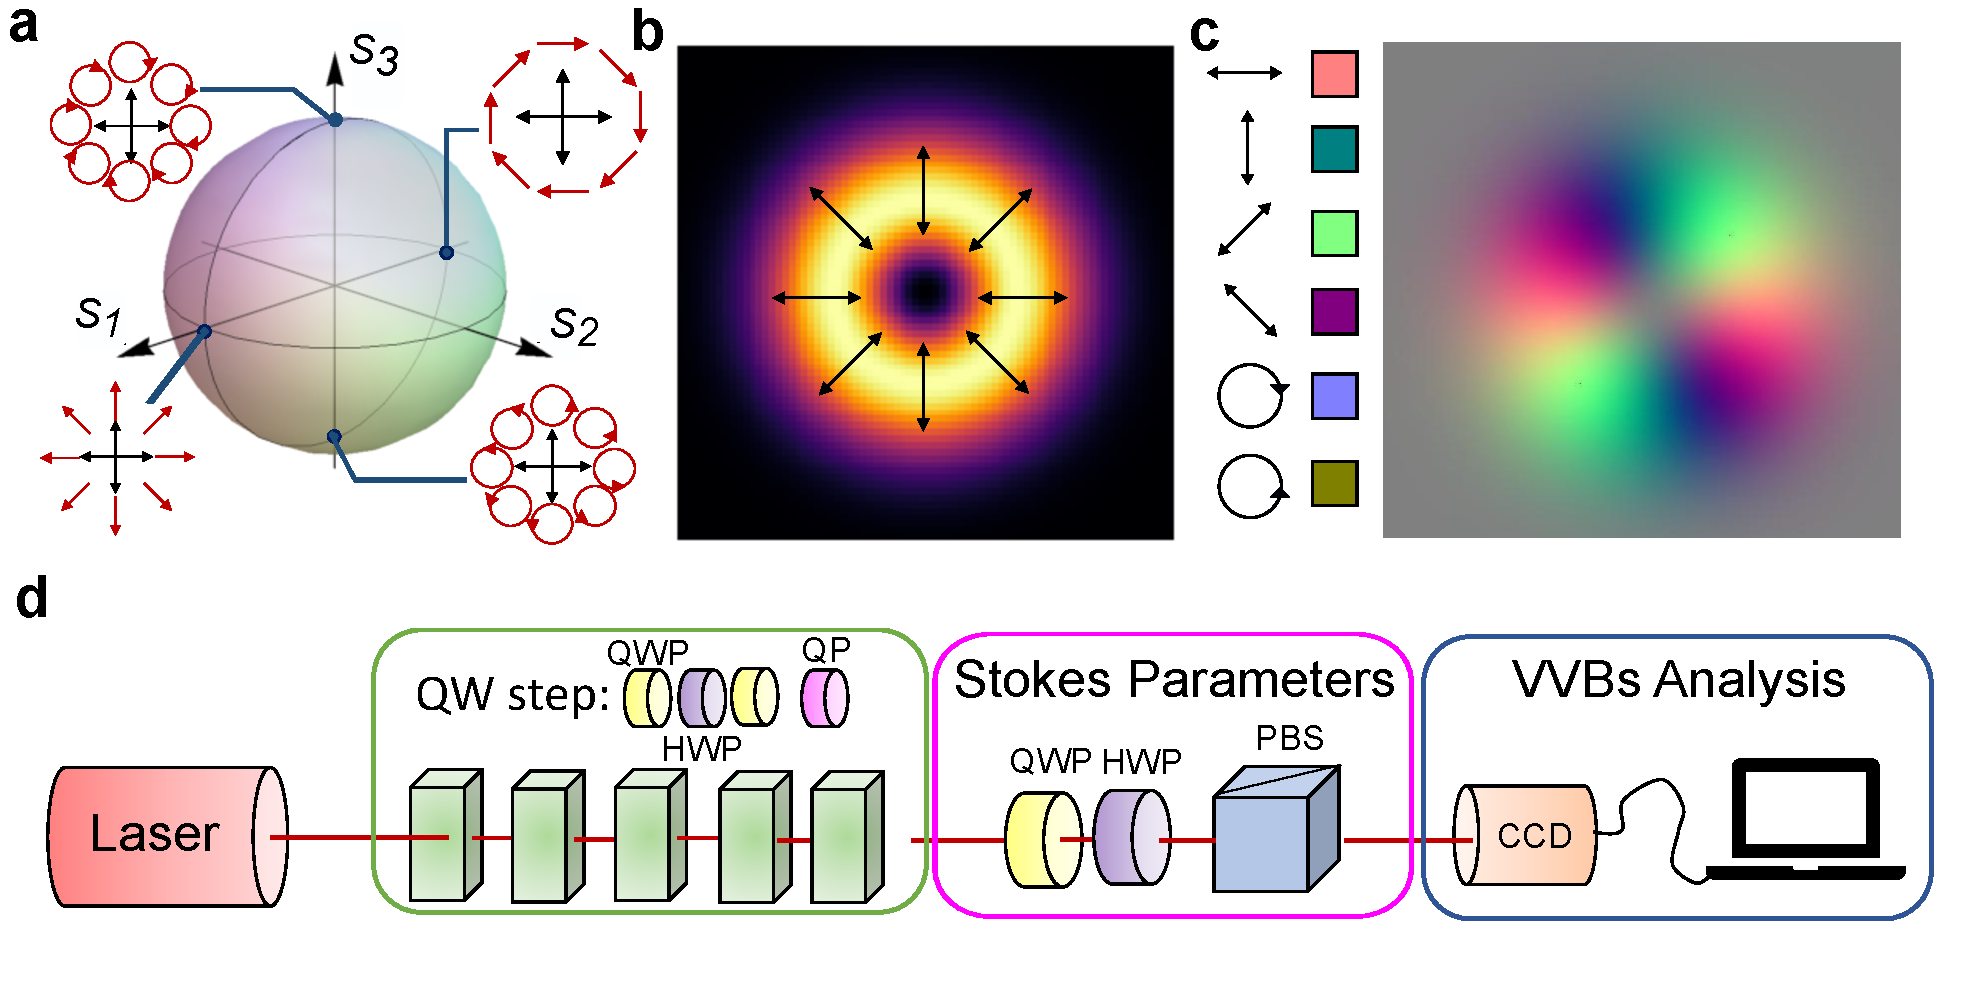
\includegraphics[width=0.8\textwidth]{VVBs-Fig1.pdf}
    \caption{
    	\textbf{(a)} High-order Poincar\'e sphere representation for $|m_{1,2}|=1$. Each point on the sphere surface corresponds to specific polarisation patterns. 
	    \textbf{(b)} A radially polarised \ac{VVB}: at a given point in the trasversal plane the polarisation vector has a different orientation. The Stokes parameters vary accordingly in the plane.
	    \textbf{(c)} Colour encoding of the polarisation pattern. 
	    The legend reports the correspondence between colours and the various polarisations.
	    On the right we have the resulting colour pattern for the VVB in panel {\bf b}.
	    Grey colour corresponds to unpolarised light.
	    \textbf{(d)} Experimental apparatus for the generation of \acp{VVB}. A continuous-wave laser emits a Gaussian beam ${\rm TEM}_{00}$ at $808$ nm. Light undergoes a 5-step quantum walk realised through a sequence of waveplates and QPs.
    	A CCD camera-based detection stage acquires information on the Stokes parameters and the polarisation pattern. Based on the intensity measured at each pixels of the  camera, Stokes parameters are evaluated and converted into RGB-coloured pictures.
    }%
    \label{fig:VVBs:poinc_sphere}
\end{figure}


\section{Experimental generation of Vector Vortex Beams}

\tmpHeading{OAM and LG modes}
\acf{OAM} states of light can be described using \ac{LG} modes.
These are solutions of the Helmholtz equation in the paraxial approximation, indexed by two integer numbers $(m, p)$, with $m$ describing the azimuthal phase structure of the beam, and $p$ its radial intensity profile.
Each \ac{LG} mode carries a set amount of \ac{OAM}, which in the single-photon regime equals $\hbar m$~\cite{allen1992orbital}.

\tmpHeading{What are VVBs?}

\tmpHeading{VVBs}
\acfp{VVB} are obtained by superposing orthogonal polarisations with different \acp{OAM}~\cite{padgett2004lights}.
More specifically, the electric field $\bs{E}_{m_1m_2p}$ of a \ac{VVB} decomposes as the sum of two~\ac{LG} modes with same $p$ and different azimuthal numbers $m_1>m_2$ carried by orthogonal polarisations:
$\bs{E}_{m_1m_2p}=\Vec{e}_L \cos{ \frac{\theta}{2}}\text{ LG$_{m_1p}$} +\Vec{e}_R e^{i \phi} \sin{ \frac{\theta}{2}}\text{ LG$_{m_2p}$}$,
where $\theta\in[0,\pi], \phi\in[0,2\pi]$ and the unit vectors $\Vec{e}_{L,R}$ stand for left and right circular polarisation, respectively.
For the purpose of this work we can ignore the radial number, setting $p=0$.
For any given value of the parameters $(m_1$, $m_2, \theta, \phi)$, the polarisation pattern of a \ac{VVB} can be mapped onto a generalised Poincar\'e sphere (cf.~\cref{fig:VVBs:poinc_sphere}). In particular, we use the higher-order Poincar\'e representation in which the poles represent eigenstates of the total angular momentum but with opposite signs~\cite{milione2011higherorder}.
These polarisation patterns are reconstructed via the \emph{Stokes parameters} $S_{j}~(j=1,2,3)$, obtained by
measuring the output intensities $I_{b_j,1},I_{b_j,2}$ associated to a given choice of polarisation basis $\{b_j \}=\{b_1=( H,V )$, $b_2=( D,A )$, $b_3=( L,R )\}$ as $S_{b_j}=(I_{b_j,1}-I_{b_j,2})/(I_{b_j,1}+I_{b_j,2})$.
%This is a way to characterise a state via its \emph{Stokes parameters} at every point of the transverse %profile.
%To do this, we first measure the output intensities $I_{b_j,1},I_{b_j,2}$ associated to a given choice of %polarisation basis $b_j$, and then compute the value of the corresponding Stokes parameter $S_{b_j}$ as %$S_{b_j}=(I_{b_j,1}-I_{b_j,2})/(I_{b_j,1}+I_{b_j,2})$.
%The canonical choice for the polarisation bases is $b_1=(H,V), b_2=(D,A)$ and $b_3=(L,R)$.
%%
For a \ac{VVB}, the values of $S_j$ depend on the coordinates in the transverse propagation plane~\cite{cardano2012polarization}.

\tmpHeading{VVBs with RGB encoding}
To visualise the polarisation patterns of \acp{VVB}, we use an RGB colour encoding in which the values of $S_j$ are interpreted as strengths of the corresponding colour. In~\cref{fig:VVBs:poinc_sphere}\textbf{b-c} we report an example of such colour encoding for radially polarised \acp{VVB}.
A natural way to generate~\acp{VVB} is using \acp{QP}~\cite{marrucci2006optical,cardano2012polarization}, which are inhomogeneous birefringent plates modifying the OAM of the incoming light conditionally to its polarisation. 
In our scheme, \acp{VVB} are generated via a sequence of polarisation-controlling waveplates interspersing $5$ cascaded QPs (cf.~\cref{fig:VVBs:poinc_sphere}\textbf{d}).
The apparatus implements a discrete-time QW in the angular momentum, where the order of LG modes takes the role of the \emph{walker} and it is changed according to the polarisation state, which embodies the \emph{coin} degree of freedom~\cite{zhang2010implementation,goyal2013implementing,cardano2015quantum,innocenti2017quantum,giordani2019experimental}.
%This apparatus implements a discrete-time QW in the OAM and polarisation degrees of freedom, in which the order of each LG mode takes the role of the \emph{walker}, and the polarisation that of the \emph{coin} degree of freedom
This allows to generate several classes of VVBs with OAM quantum numbers taking odd values in the interval $\{-5,..,5\}$.
We then collect images associated with different \acp{VVB} and use them to train and benchmark our ML-based approaches to classification , as discussed in the next sections.


\tmpHeading{State engineering scheme}
We use the same experimental platform presented in~\cref{chapter:experimental_engineering_qudits}, with $5$ \acp{QP} in cascade that can be interspaced by either \acp{HWP} or \acp{QWP}. 
% The HWPs compensate the polarisation flip operated by the QPs for the generation of higher order \ac{LG} modes. Conversely, the QWP acts on circular polarisations as an Hadamard transformation. 
Using different sets of these waveplates between consecutive QPs, we can generate VVBs corresponding to different pairs $(m_1,m_2)$ of OAM quantum numbers, and parameters $(\theta, \phi)$.
%sof the higher the increases the \ac{OAM} values associated to a \ac{VVB}. Moreover, using quarter waveplates it is possible to generate \acp{VVB} characterised by Laguerre Gauss modes with different azimuthal numbers $m_{1}>m_{2}$.


\tmpHeading{How are images collected?}
The experimental images are collected using a \ac{CCD} with a resolution of $1360 \times 1024$. 
However, we note that a resolution of $128 \times 128$ is already sufficient for the classification tasks we consider. Indeed, the training stage of the algorithms can be significantly speeds up by coarse-graining the images via an integration of its sub-blocks without any loss of information. 

\tmpHeading{Stokes parameters}
For each generated \ac{VVB}, we measure the transverse intensity profile corresponding to each of the two outputs associated with each one of the three independent polarisation bases: $b_1=(H,V), b_2=(D,R)$, and $b_3=(L,R)$, where $\ket L\equiv \frac{1}{\sqrt2}(\ket H + \ket V)$, $\ket R\equiv \frac{1}{\sqrt2}(\ket H - \ket V), \ket D\equiv \frac{1}{\sqrt2}(\ket H + i \ket V), \ket R\equiv \frac{1}{\sqrt2}(\ket H - i \ket V)$.
This amounts, for each generated \ac{VVB}, to acquiring six intensities for each pixel of the \ac{CCD}. This representation is however redundant, as the properties of the VVBs only depend on the relation between the two intensities in each polarisation basis (which, in the single-photon regime, would correspond to the two outcome probabilities).
We therefore represent states using the \emph{higher-order Poincar\'e representation} \cite{milione2011higherorder,cardano2012polarization}. In this representation, each state is mapped into its three \emph{Stokes numbers} $S_{b_j}$, which equal the difference between the two intensities in each choice of polarisation basis:
\begin{equation}
  S_{b_j} = \frac{I_{b_j,1} - I_{b_j,2}}{I_{b_j,1} + I_{b_j,2}},
\end{equation}
where $b_j$ is one of the three canonical polarisation bases, and $I_{b_j,1}, I_{b_j,2}$ are the intensities corresponding to the two possible outcomes when measuring in the basis $b_j$.
In this representation, we therefore associate three real numbers to each each pixel in the \ac{CCD} camera. This means that each detected state is characterised by $128\times128\times3$ real numbers. To visualise these states, we represent the three Stokes numbers $S_{b_j}$ using an RGB colour encoding. In particular, the strengths of the colours red, green and blue are associated with the $S_{1}$, $S_{2}$ and $S_{3}$ parameters,  respectively.
This allows us to map each VVB state into a three-channel coloured image.

For the purpose of the classification algorithms described in~\cref{sec:VVBs:classification,sec:VVBs:dimensionality_reduction,sec:VVBs:SVMs}, each state is represented as a real vector of length $128\times128\times 3$.


\begin{figure}[tb]
	\centering
	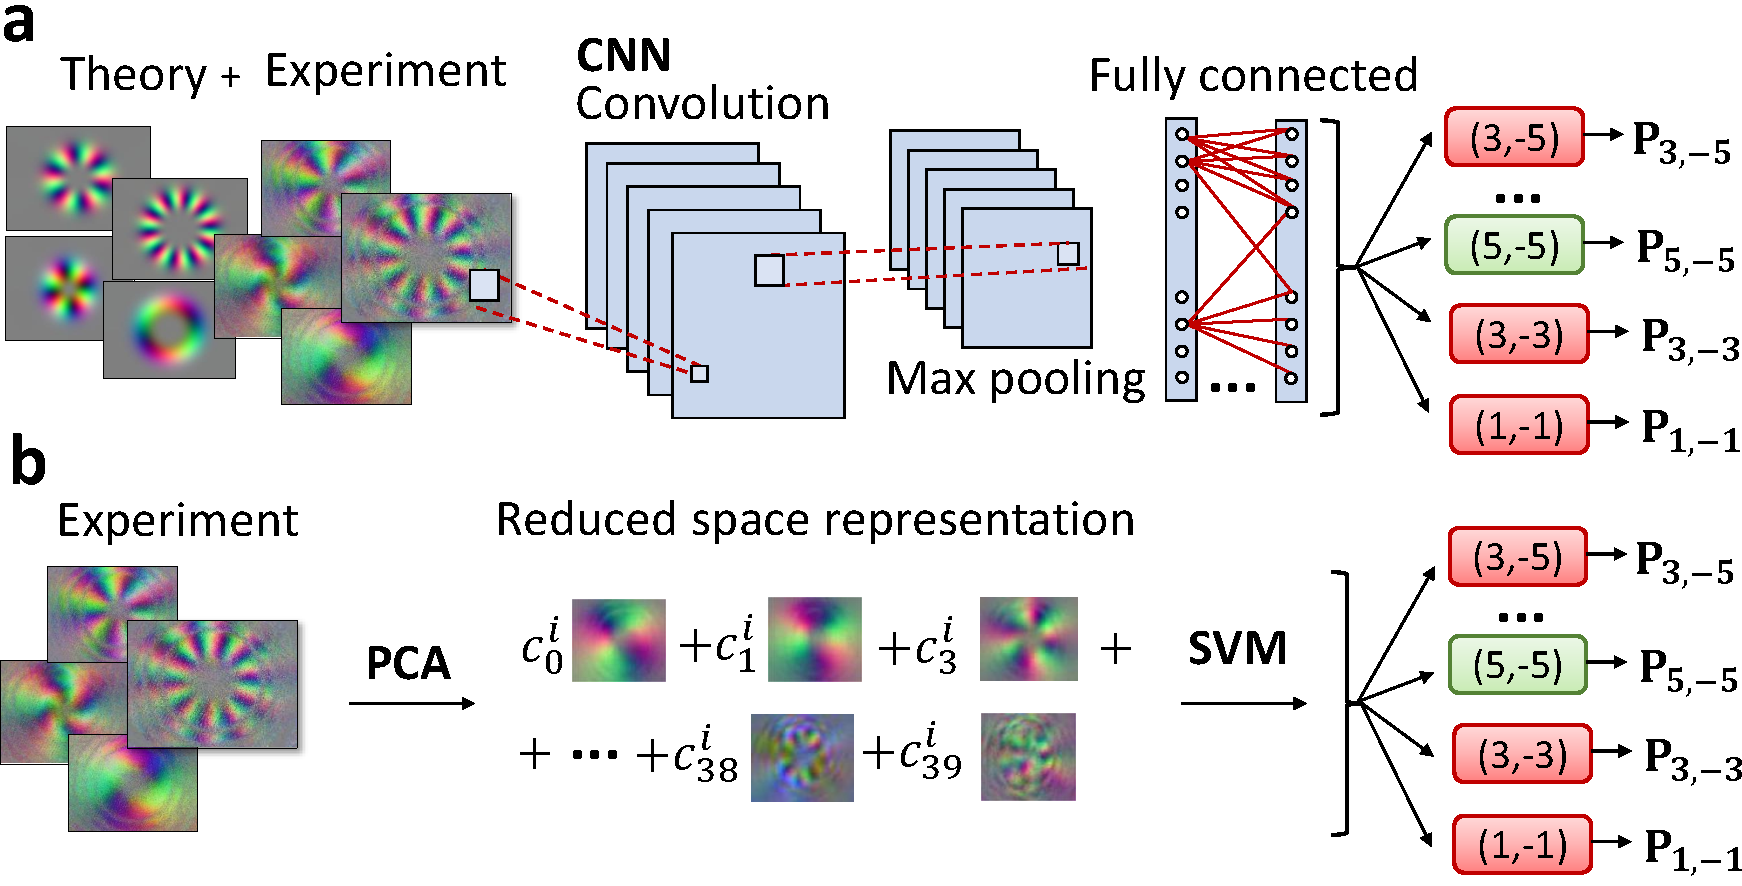
\includegraphics[width=\textwidth]{conc_VVB_2.pdf}
	\caption{
	\textbf{(a)}
	Working principles of \acp{CNN}. The training set consists of a series of simulated images, plus some others collected from the experimental platform.
	\textbf{(b)}
	Classification scheme using linear \ac{PCA}.
	After reducing the dimensionality of the dataset via \ac{PCA}, a linear \ac{SVM} is used to classify experimental images. 
	}
	\label{fig:VVBs:class_techniques}
\end{figure}

\begin{figure}[tb]
    \centering
    \includegraphics[width=0.8\textwidth]{VVBs-Fig3.pdf}
    \caption{
	    \textbf{(a)} Comparison between expected and recorded polarisation patterns for some \acp{VVB} of the ensemble in table, with the corresponding values $(m_1,m_2)$.
	    \textbf{(b)} Scaling of the average accuracy per class when classifying states into one of the $15$ VVB classes,
	    against the fraction of experimental images in the training set. 
	    Inset: best truth table.
	    Rows (columns) stand for the possible $(m_1,m_2)$ pairs (as assigned by the CNN). The matrix elements have been averaged over $100$ experimental images per class.
    }%
    \label{fig:VVBs:resultsCNN}
\end{figure}



\section{Convolutional neural networks}
\label{sec:VVBs:CNNs}

\tmpHeading{What do we use CNNs for?}
We show here how to train a \ac{CNN} to retrieve the parameters $(m_1,m_2)$ characterising a given VVB from experimentally measured Stokes parameters.
This means to feed the algorithm with input images corresponding to one of a number of possible classes of states, and train the network to give as output the corresponding value of the OAM numbers $(m_1,m_2)$.
Moreover, we train the network to recognise the parameters $(\theta,\phi)$ for a given measurement of Stokes parameters, when all the input states have the same OAM numbers $(m_1,m_2)$.

\tmpHeading{What are CNNs?}
\acp{CNN} are translation-invariant deep NNs well-suited for image classification~\cite{lecun2015deep}, to recognise off-centre images and segmented handwritten digits~\cite{simard2003best,ciresan2011flexible},
and for facial recognition tasks~\cite{matsugu2003subject}. 
In their simplest form, \acp{CNN} work by first applying a \emph{convolutional layer}, which consists of a series of nonlinear transformations applied to the input images, followed by a \emph{max-pooling layer}, which downsamples and filters the information extracted by the previous layer. Finally, a fully connected layer functions as a \emph{classifier}, categorising the information extracted in the previous layers into one of a small number of possible output categories.

\tmpHeading{CNNs more in detail}
We describe here in more detail the structure of the \ac{CNN} used to classify the experimental images.
In a standard \ac{CNN}, the convolution in a particular location $(x,y)$ is obtained by computing the inner product between a $k \times k$ sub region of the input image and a filter of the same size. Repeating this process for each location on the input image, it is possible to obtain an activation map associated to specific features. Typically, more than one filter is used in one convolution layer and $N$ features are extracted.
A max-pooling layer is used immediately after the convolutional layer to reduce the number of parameters. The output of the previous layer are then divided into blocks of size $p \times p$, and the $\max$ function is applied over each block.
Finally, a fully connected layer classifiers the data by determining which features are most correlate to a particular class.
At the beginning, the filters of the features extractors are randomly initialised. Consequently, they are computed via a back-propagation process to optimise the classification of a training set.

\tmpHeading{Categorisation into discrete classes}
The network is first fed with a training set made out of simulated images of \acp{VVB} achievable with a five-step \ac{QW}.
The task is then to discern between $15$ classes, corresponding to the pairs $(m_1,m_2)$ in Fig.~\ref{fig:VVBs:resultsCNN}\textbf{a}.
For each class we generate states with $\theta=\pi/2$ and $\phi\in[0,2\pi]$. The size of the training set is $400$ images per class. Additional $100$ simulated images per class are used to benchmark the performance during training. In these conditions, the network achieves an accuracy of $100\%$. 
We then collect $100$ experimental images per class, to use as new validation set (cf. Fig.~\ref{fig:VVBs:class_techniques}{\bf a}). Fig.~\ref{fig:VVBs:resultsCNN}{\bf a}-{\bf b} shows the mean accuracy per class against the fraction of experimental images gradually inserted in the training set, starting from one consisting of computer-generated images only.
Remarkably, a small increase of the number of experimental images in the training set results in a good accuracy reached by the network (cf. Fig.~\ref{fig:VVBs:resultsCNN}{\bf b}): an average accuracy of $\sim 0.989$ is already obtained when $12.5\%$ of the training set is composed of experimental images.


\tmpHeading{Retrieving the position in the Poincaré sphere}
We use a similar approach to retrieve the position on the Poincaré sphere corresponding to states generated with fixed $(m_1,m_2)$.
We then test the performance of the CNN in the classification of each recorded VVB according to the values $(\theta,\phi)$ for $m_2=-m_1=1$.
To achieve this, the network should discriminate rotations in the polarisation patterns (i.e. changes in $\phi$) and variations in the colour tone (i.e. changes in $\theta$). A drawback of using any type of classifier for this task is that VVBs with $|m_i|\gg1$ display a polarisation pattern whose periodicity decreases as $\frac{2\pi}{|m_1-m_2|}$ (cf. Fig.~\mbox{\ref{fig:VVBs:resultsCNN}}{\bf a})~\cite{fickler2012quantum,dambrosio2013photonic}.
This complicates the recognition of $\phi$, as changes in the phase generate only small rotations of the pattern.
Furthermore, the classification of the VVB on the sphere requires a discretisation of $\theta$ and $\phi$, which results in dividing the sphere in sectors. This means that VVBs placed at the borders of these intervals are more difficult to assign to a specific class.
The network is then trained with simulated images corresponding to different positions on the sphere. 
%(that is, different values of $(\theta,\phi)$).
The latter is divided in 26 sectors as follows: $\theta$ is divided in $3$ intervals $\left[k \frac{\pi}{8}, (k+2) \frac{\pi}{8}\right]$ ($k=2n+1$, $n \in \{0,1,2\}$), while $\phi$ is split in the 8 classes $\left[t \frac{\pi}{4}, (t+1) \frac{\pi}{4}\right]$ with $t \in \{0,...,7\} $. The remaining two classes, representing the two poles, correspond to $\theta \in \left[0, \frac{\pi}{8}\right]$ and $ \left[ \frac{7}{8} \pi, \pi\right]$, with no distinction in $\phi$ [cf. Fig. \ref{fig:VVBs:PCAresults}{\bf a}].
We generate $500$ images per class in the training set, and $125$ per class for the validation one. The maximum accuracy  achieved is $\sim 0.90$. This result, which is inferior with respect to what is achieved by only inferring $m_{1,2}$,  confirms the sub-optimality of the method when we had to artificially coarse-grain two continuous parameters.

\tmpHeading{How did we implement the CNN?}
To build and train the \ac{CNN} we used the Python library \emph{Keras}~\cite{chollet2015keras}.
We used a CNN with three feature extractors and one classifier. In each convolution layer we apply $32$ filters of size $3 \times 3 \times 3$ and as activation function is used the Rectified Linear Unit (ReLU). Subsequently, the max function is applied over blocks of size $2 \times 2 \times 3$  in max-pooling layers. %\redComm{(unclear)}. 
The final classification is performed by a fully connected layer which uses a sigmoid activation function. The network training consists of a finite number of epochs each of which composed of $200$ training steps and $100$ validation steps. 


\section{Dimensionality reduction}
\label{sec:VVBs:dimensionality_reduction}

\tmpHeading{What do we use DR for?}
We now present an alternative approach to classify \acp{VVB} from experimental data, leveraging \ac{DR}.


\subsection{Dimensionality Reduction and Principal Component Analysis}

\tmpHeading{What is DR?}
\acf{DR} is a class of algorithms whose goal is to find low-dimensional encodings of high-dimensional datasets~\cite{cunningham2008dimension,fodor2002survey}.
This can have several advantages, from easing data visualisation, to improving the efficiency of classification and regression algorithms, which can be applied on the reduced representation of the data.

\tmpHeading{PCA}
A classical \ac{DR} algorithm is \acf{PCA}.
In its simplest form, \ac{PCA} is a \emph{linear} \ac{DR} algorithm which, given a dataset of vectors in some high-dimensional space $\RR^n$, finds the directions which capture the maximum amount of information about the dataset~\cite{jolliffe2011principal,jolliffe2016principal}.
More specifically, given a dataset comprised of $N$ real vectors of length $M$, we define the \emph{data matrix} $\bs X$ as the $N\times M$ matrix whose $i$-th row is the $i$-th dataset vector. \ac{PCA} then finds the vectors $\bs a\in\RR^{M}$ that maximise the variance of $\bs X\bs a$. This turns out to be equivalent to diagonalising $\bs S\equiv \tilde{\bs X}^T\tilde{\bs X}/(N-1)$, where $\tilde{\bs X}$ is the \emph{centered data matrix}, which is equal to $\bs X$ modulo each of its columns shifted in order to average to zero.
The first $k$ \emph{principal components} found by \ac{PCA} are then the $k$ eigenvectors of $\bs S$ corresponding to the largest $k$ eigenvalues.
Note that these principal components are themselves vectors of the same ``type'' as the data vectors. This means that \ac{PCA} effectively generates a set of data vectors which ``optimally represent'' the information content of the given dataset.

\tmpHeading{PCA and VVBs}
The rationale behind using \ac{PCA} in the context of \acp{VVB} is that, although experimental images live in extremely high-dimensional spaces (whose dimension is of the order of the number of pixels in the \ac{CCD} camera), the underlying dimension of the generated \acp{VVB} is typically much lower.
This means that, although the experimental dataset might \emph{a priori} seem like a complicated bundle of high-dimensional vectors, the underlying data is actually characterizable by a small number of parameters. Furthermore, the linearity of the mapping from the full to the reduced space makes it preserve many of its geometrical properties.
This is a form of \emph{unsupervised} learning, as we gain useful information about the origin of the images are inferred without feeding the algorithm with any knowledge of the underlying process.


\tmpHeading{For example...}
For example, in our case, each row of $\bs X$ is a vector of length $128\times128\times3$ containing the Stokes parameters $S_{b_1}, S_{b_2}, S_{b_3}$ for each pixel of the camera.
Because each image corresponds to such a vector, and vice versa each such vector corresponds to the image of a \ac{VVB}, we can represent the principal components found by \ac{PCA} again in the form of images, which allows us to gain some intuition into the type of principal components that optimally represent the data according to \ac{PCA}.


\subsection{Retrieving states from probabilities}

\tmpHeading{Measuring in a single measurement basis}
Collecting experimental intensity images with the \ac{CCD} camera is akin to collecting the statistics associated to measuring a specific state in a fixed measurement basis. Despite this not being, in general, sufficient to reconstruct a quantum state, it can be when some assumptions on the input state or the type of measurement~\cite{banchi2018multiphoton}.
More specifically, let $\rho$ be the density matrix characterising the state. The corresponding observed statistics in a chosen measurement basis is given by the set of probabilities
\begin{equation}
	p_k = (\calU\rho\calU^\dagger)_{kk}
	    = \sum_{ij}\calU_{ki}\bar\calU_{kj}\rho_{ij},
\end{equation}
for some unitary $\calU$.
This means that the mapping between density matrices and detected probabilities is linear: $\bs p=\Psi(\rho)$ for some linear map $\Psi$. This implies that many geometrical features of the space of states is preserved in the probabilities space. Moreover, a suitable choice of $\Psi$ will allow to retrieve $\rho$ from the knowledge of $\bs p$.
For this to be possible, $\Psi$ needs to have a number of rows greater than or equal to the number of columns. Physically, this amounts to the measurement basis containing a sufficient number of elements. More specifically, $\Psi$ needs to be \emph{left-invertible}, which is the case when its columns are linearly independent.


\tmpHeading{Application to experimental VVB images}
In our case, $\rho$ is a description of a VVB in the OAM-polarisation basis, while $\calU$ is the unitary mapping this basis into the position basis, which is the one that CCD cameras naturally operate on. In principle, one might need to take care of the different dimensionalities of these two spaces (the OAM space is countable while the position one is not), but this is easily fixed by discretising the position space, which is what is done naturally by the finite number of pixels of the CCD camera. 
In other words, $\rho$ describes the state in the OAM-polarisation basis, which is the basis in which the generated states are efficiently described, whereas $\calU\rho\calU^\dagger$ describes the same state in the position basis, which is the one in which the CCD camera operates on.
The set of detected probabilities is then given by $\bs p=\on{diag}(\calU\rho\calU^\dagger)\equiv\Psi(\rho)$,
where $\Psi$ is defined as the linear map that sends $\rho$ to the set of measured probabilities $\bs p$.
It should be noted that, while here we use a formalism and vocabulary evocative of quantum states, the states actually used in the experiment are classical. This in no way impacts the formal description of the protocol, and the only thing that should change when the states used are classical is that the probabilities $\bs p$ should be reinterpreted as intensities.
Crucially, the linearity of $\Psi$ implies that it preserves the \emph{convexity} of the space of states, and therefore many of its geometrical features.
For example, if we consider the set of states of the form $c_0 \ket{\uparrow,m=m_1} + c_1 \ket{\downarrow,m=m_2}$ with $m_1\neq m_2$, then the associated density matrices will be arranged to form a three-dimensional sphere embedded in the full state space (because these are effectively different states of a single qubit).
Thanks to the linearity of $\Psi$, \emph{the corresponding probabilities $\bs p$ will also be contained in a spherical surface}, up to possible rescaling of the axes.
In other words, the Bloch sphere of the original two-dimensional system is still present, albeit hidden, in the experimental images, embedded into an extremely high-dimensional space.


\begin{figure}[tb]
    \centering
    \includegraphics[width=0.8\linewidth]{VVBs-Fig4.pdf}
    \caption{
		\textbf{(a)} High order Poincar\'e sphere for \acp{VVB} with $|m_{1,2}|=1$. Magenta-coloured parallels (Blue-coloured meridians) mark intervals between consecutive values of $\theta$ ($\phi$). 
		Along a meridian the colours of the pattern vary from the hottest to the coldest one. Along a parallel, the patterns rotate. 
		\textbf{(b)}
		Comparison between experimental and simulated \ac{VVB} images for different angles $(\theta, \phi)$.
		\textbf{(c)}
		Distribution of fidelities obtained comparing each experimental VVBs with its reduced 3D representations given by PCA. Projecting each image onto its first three principal axes and rescaling brings the data (orange points) onto a sphere in 3D, as shown in the inset. The inner (outer) black (semi-transparent) sphere is added for contrast [radius equal to that of the point with smaller (larger) radius].
		\textbf{(d)}
		Average prediction accuracy of a linear \ac{SVM} classifier, trained and tested after applying linear DR to the data, against the number of reduced dimensions $n_c$.
		For each of the 15 classes (cf.~\cref{fig:VVBs:resultsCNN}a) in which the experimental dataset was divided, we show in the inset the true-table. 
    }%
    \label{fig:VVBs:PCAresults}
\end{figure}


\subsection{Results}

\tmpHeading{PCA applied to experimental data}
As a notable example, we apply these observations to VVBs with $m_2=-m_1=1$, which can be pictured as lying on a sphere, in the higher-order Poincaré representation. 
of the form $c_0 \ket{L,m=1} + c_1 \ket{R, m=-1}$ with $\abs{c_0}^2+|c_1|^2=1$.
The inclusion of only two orthogonal basis states makes these states effectively equivalent to a single qubit. 
Indeed, \ac{PCA} applied to the experimental dataset of~\cref{fig:VVBs:PCAresults}\textbf{b}, 
reveals that only three directions capture most of the information content of the images. Projecting the images along these three principal components, we recover that the data is arranged in the form of a three-dimensional sphere embedded in the high-dimensional space of experimental (cf. inset of~\cref{fig:VVBs:PCAresults}\textbf{c}).
Remarkably, this was not obvious from the experimental dataset alone, but was easily found via \ac{DR}. This result highlights the potential of \ac{DR} to  reveal features of the underlying states generating a given experimental dataset, also in the presence of experimental noisy conditions.
To assess the accuracy of such reconstruction, we compute the average fidelity $\mathcal F_{\text{avg}}$ between the expected state and the one found by our analysis with PCA. As shown in the histogram of Fig.~\ref{fig:VVBs:PCAresults}c,  this is found to be $\mathcal F_{\text{avg}}\sim0.96$ (standard deviation $\sim0.01$), thus certifying the quality of the reconstruction.

\begin{figure}[tb]
  \centering
  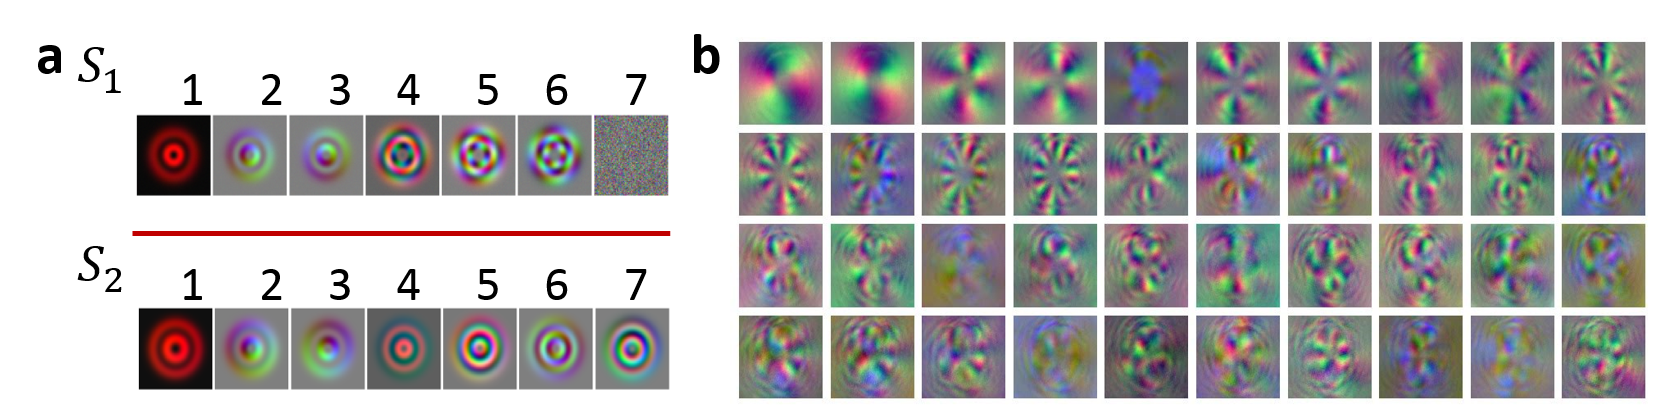
\includegraphics[width=0.98\textwidth]{S1_fig.png}
  \caption{
      \textbf{a,}
       Principal components obtained using PCA on simulated datasets of noisy VVB. The first (second) row shows the first seven principal components obtained on the dataset $\mathcal S_1$ ($\mathcal S_2$). 
       The first 6 (all 7) components correspond to non-vanishing singular values.
       \textbf{b,} First 40 principal components individuated in the experimental dataset corresponding to the 15 classes labelled by $(m_1,m_2)$, discussed in the main text.%
    }
    \label{fig:S1}
\end{figure}


\tmpHeading{Toy examples of application of PCA to VVBs}
To see the usefulness of these ideas to understand the type of states generated by a given apparatus, we consider here two examples of applications of \ac{PCA} for different types of input states. 
In all of these cases, \ac{PCA} is applied without any previous knowledge of the type of states that underly the observed experimental images, and is therefore to be considered a type of \emph{unsupervised learning}.
Consider a simulated set of images corresponding to VVBs of the form
$c_1\ket{L,m=1}+c_2\ket{R,m=2}$ and
$c_1\ket{L,m=1}+c_2\ket{R,m=4}$, where the coefficients $c_i$ are sampled uniformly at random from the set of $c_{1},c_2\in\mathbb{C}$  such that $|c_1|^2+|c_2|^2=1$ (\emph{i.e.} uniformly sampled on the Bloch sphere).
Applying PCA to this dataset, we find six non-vanishing singular values, whose associated principal components are given in Fig.~\ref{fig:S1}a.
This is consistent with the dimension of the subspace  spanned by states of the form $\mathcal S_1=\{c_1\ket{L,1}+c_2\ket{R,2}, c_3\ket{L,1}+c_4\ket{R,4}\}$,  as the set of corresponding density matrices is spanned by the six orthogonal matrices
$X^{(1,2)}, X^{(1,4)}, Y^{(1,2)},Y^{(1,4)},Z^{(1,2)}\pm Z^{(1,4)}$, where $X^{(i,j)}=\ketbra{i}{j}+\ketbra{j}{i}$ is the Pauli $X$ matrix acting on the $(i,j)$ subspace, and similarly for $Y^{(i,j)}$ and $Z^{(i,j)}$.
On the other hand, if the dataset under consideration consists of states of the form $\mathcal S_2=\{c_1\ket{L,1}+c_2\ket{R,2}, c_3\ket{L,3}+c_4\ket{R,4}\}$, then \ac{PCA} finds \emph{seven} principal components associated with non-vanishing singular values (see Fig.~\ref{fig:S1}a).
This is consistent with the underlying state space being spanned by the seven orthogonal Hermitians:
\begin{equation}
\begin{gathered}
    X^{(1,2)}, \,\, X^{(3,4)}, \,\,
    Y^{(1,2)}, \,\, Y^{(3,4)}, \\
    Z^{(1,2)},\quad
    -Z^{(1,2)} + 2 Z^{(1,3)}, \\
    -Z^{(1,2)} - Z^{(1,3)} + 3 Z^{(1,4)}.
\end{gathered}
\end{equation}
These matrices can be obtained by direct analysis of the type of states contained in $\mathcal S_2$ and then finding a set of orthogonal Hermitian matrices generating the corresponding set of density matrices.
It is worth noting how this method provides a quick and easy way to gain useful information about the dimensionality of generated states, as well as about other properties such as specific symmetries, which, as shown in~\cref{fig:S1}, are often picked up by the principal components.


\section{Support vector machines}
\label{sec:VVBs:SVMs}

\subsection{What are they?}

\tmpHeading{What are SVMs?}
\acfp{SVM} are a class of \emph{supervised learning} algorithms, whose goal is to classify data by finding an optimal partition of the feature space such that all the vectors with the same training label lie on the same classification sector.
In particular, \emph{linear} \acp{SVM} try to separate the data linearly, that is, look for an optimal separating hyperplane.

\tmpHeading{The math of linear SVMs}
A SVM takes as input a training set of labelled data of the form $\{(\bs x_1,\ell_1),...,(\bs x_n,\ell_n)\}$ where $\bs x_i\in\RR^N$ and $\ell_i$ is one of two possible labels, $N\in\NN$ being here the dimension of the feature vectors. If there are only two possible labels, we can conventionally assume $\ell_i\in\{-1,1\}$.
The goal is to find a linear separation, which is characterised by two parameters $\bs w$ and $b$ which identify an hyperplane as the set of $\bs x\in\RR^N$ such that $\bs w\cdot\bs x=\bs b$. We want this hyperplane to be such that, for all training vectors $\bs x_i$, the constraint $\ell_i(\bs w\cdot\bs x_i-\bs b)\ge1$ is satisfied.
New data is then categorised using the \emph{classifier} $g_{\bs w,\bs b}(\bs x)=2\Theta(\bs w\cdot\bs x-\bs b)-1$, which equals $\pm1$ depending on whether the point $\bs x$ is on one side or the other of the separation determined by $\bs w,\bs b$.
This is the so-called \emph{hard-margin} SVM, because this is only possible if every single training point is strictly on one or the other side of the separating hyperplane.
An often more practical alternative are the so-called \emph{soft-margin} SVMs, in which this strict requirement is lifted. Instead, the goal becomes to minimise the average value of
$\max(0, 1- \ell_i (\bs w\cdot\bs x_i-\bs b))$, trying at the same time to keep $\|\bs w\|$ as low as possible. This variation makes the algorithm more robust and able to classify data even in the presence of some noise \highlight{(an example with figures of hard- vs soft-margin classification would be nice)}.


\subsection{How do we use them?}

\tmpHeading{SVMs after PCA}
We now show how the reduced representations provided by \ac{PCA} can function as starting point to train a classifier with an accuracy comparable with that of the \acp{CNN} used in~\cref{sec:VVBs:CNNs}, whilst requiring a drastically reduced amount of computational resources.
More precisely, we use as classifiers linear multiclass \acp{SVM}~\cite{hearst1998support,shawe2000support}. These supervised learning algorithms categorise data by finding the hyperplane that optimally separates the training dataset in accordance with the corresponding labels.
We use here in particular a \emph{linear}, multiclass \ac{SVM}, whose goal is to find hyperplanes in the feature space that optimally separate the datapoints corresponding to different classes.
During the training phase, a set of training experimental images is used to find the separating hyperplanes, which is then used to classify new experimental images.
% Both training and classification are performed \emph{after} the dimensionality reduction has been carried out via \ac{PCA}. This makes for improved computational times as well as making the algorithm more robust to experimental noise and imperfections.

\tmpHeading{What do we use the SVMs for?}
As done for the \ac{CNN}, we consider the task of classifying experimental dataset of VVBs. We train a \ac{SVM} on the reduced space obtained via \ac{PCA}, applied to the experimental dataset reported in~\cref{fig:VVBs:resultsCNN}\textbf{a}. This stage significantly improves the training cost of the classifier since the latter will work on a synthesised description of the high-dimensional space of images in which the features of each class can be easily recognised.
This not only significantly speeds up the training stage, but also makes for a more robust classification, thanks to the property of dimensionality reduction algorithms to weed out statistical and experimental noise.
What's more, the geometrical picture offered by the reduced representation tells us when we should expect this classification to be accurate: \ac{PCA} effectively retrieves the description of the states in the generalised Bloch representation, therefore the classification will give good results whenever the states are linearly separated in state space.


\tmpHeading{What is used for the training?}
The~\ac{SVM} was trained on half of the experimental data, with the other half used to test the resulting accuracy. A breakdown of the classification performance is reported in the inset of~\cref{fig:VVBs:PCAresults}\textbf{d}, where we detail how the images belonging to each class were classified.

\tmpHeading{What kind of SVM do we use?}
We used here a \emph{linear} SVM, instead of a commonly used SVM with RBF kernel, because we found it to perform better: an RBF kernel was found to give, in our case, an average accuracy of only $\sim94\%$.
Furthermore, in~\cref{fig:VVBs:PCAresults}\textbf{d} we highlight how the average overall accuracy depends on the dimension of the reduced representation: $\sim 25$ dimensions are already sufficient to get good average accuracies.

\subsection{Results}

The average classification accuracy achieved on images not included in the training set is $\sim 98 \%$. This result confirms that the description provided by \ac{PCA} is sufficient to capture the important features of the generated states, thus allowing for a dramatically more efficient classification scheme.


\section{Conclusions}
\label{sec:VVBs:conclusions}

We presented a new approach to classify \acp{VVB} leveraging ML techniques. We demonstrated how the use of inference strategies based on CNNs and PCA (enhanced by SVMs) allows to extract efficiently properties of high-dimensional photonic \ac{VVB} systems.
In particular, DR was used to obtain a deeper understanding of the underlying geometrical properties of the experimentally generated states, without requiring prior knowledge about the physics of the generation apparatus.
% this is not quite right
By embedding a variety of {\ac{ML}} algorithms into our experimental pipeline, the task of characterising structured light is made significantly broader in the methods, ranging from supervised to unsupervised learning, and more flexible in the applications, classification and regression tasks.
%
%Then, the investigation of different techniques in the ML field has provided a more general framework for the characterization of structured light. 
% 
While paving the way to further experimental validations -- potentially also in experimental settings that do not rely on optical networks -- we believe that numerous tasks of relevance to modern photonics could benefit from introducing similar {\ac{ML}} ideas into their characterisation protocols. These techniques can prove to be useful add-on to tasks ranging from the design of automatised approaches to the characterisation of experimental platforms and experiments, to the provision of solutions to OAM demultiplexing in the context of classical and quantum communication and, more generally, for the use of structured light in quantum technologies.

\textit{Note--} During the reviewing process of this manuscript, the authors
became aware of a related work~\cite{liu2019superhighresolution} addressing a similar topic.
